\documentclass[]{jarticle}          % 一段組
%\documentclass[twocolumn]{jarticle} % 二段組

\textwidth 180mm
\textheight 255mm
\oddsidemargin -12mm
\topmargin -15mm
\columnsep 10mm

%\vspace{0.5cm} % 一段組の場合はコメントアウトした方が体裁がよいx
%] % 一段組の場合はコメントアウトする

\usepackage{styles/labheadings}
\usepackage[dvipdfmx]{graphicx,color}
\usepackage{amsmath,amssymb}
\usepackage{url}
% 追加
\usepackage{listings,jvlisting} 
\usepackage[hang,small,bf]{caption}
\usepackage[subrefformat=parens]{subcaption}
\usepackage{indentfirst}
\captionsetup{compatibility=false}

\newcommand{\aU}{\mbox{\boldmath $a$}}
\newcommand{\bU}{\mbox{\boldmath $b$}}
\newcommand{\cU}{\mbox{\boldmath $c$}}
\newcommand{\dU}{\mbox{\boldmath $d$}}
\newcommand{\eU}{\mbox{\boldmath $e$}}
\newcommand{\fU}{\mbox{\boldmath $f$}}
\newcommand{\gU}{\mbox{\boldmath $g$}}
\newcommand{\hU}{\mbox{\boldmath $h$}}
\newcommand{\iU}{\mbox{\boldmath $i$}}
\newcommand{\jU}{\mbox{\boldmath $j$}}
\newcommand{\kU}{\mbox{\boldmath $k$}}
\newcommand{\lU}{\mbox{\boldmath $l$}}
\newcommand{\mU}{\mbox{\boldmath $m$}}
\newcommand{\nU}{\mbox{\boldmath $n$}}
\newcommand{\oU}{\mbox{\boldmath $o$}}
\newcommand{\pU}{\mbox{\boldmath $p$}}
\newcommand{\qU}{\mbox{\boldmath $q$}}
\newcommand{\rU}{\mbox{\boldmath $r$}}
\newcommand{\sU}{\mbox{\boldmath $s$}}
\newcommand{\tU}{\mbox{\boldmath $t$}}
\newcommand{\uU}{\mbox{\boldmath $u$}}
\newcommand{\vU}{\mbox{\boldmath $v$}}
\newcommand{\wU}{\mbox{\boldmath $w$}}
\newcommand{\xU}{\mbox{\boldmath $x$}}
\newcommand{\yU}{\mbox{\boldmath $y$}}
\newcommand{\zU}{\mbox{\boldmath $z$}}
\newcommand{\AU}{\mbox{\boldmath $A$}}
\newcommand{\BU}{\mbox{\boldmath $B$}}
\newcommand{\CU}{\mbox{\boldmath $C$}}
\newcommand{\DU}{\mbox{\boldmath $D$}}
\newcommand{\EU}{\mbox{\boldmath $E$}}
\newcommand{\FU}{\mbox{\boldmath $F$}}
\newcommand{\GU}{\mbox{\boldmath $G$}}
\newcommand{\HU}{\mbox{\boldmath $H$}}
\newcommand{\IU}{\mbox{\boldmath $I$}}
\newcommand{\JU}{\mbox{\boldmath $J$}}
\newcommand{\KU}{\mbox{\boldmath $K$}}
\newcommand{\LU}{\mbox{\boldmath $L$}}
\newcommand{\MU}{\mbox{\boldmath $M$}}
\newcommand{\NU}{\mbox{\boldmath $N$}}
\newcommand{\OU}{\mbox{\boldmath $O$}}
\newcommand{\PU}{\mbox{\boldmath $P$}}
\newcommand{\QU}{\mbox{\boldmath $Q$}}
\newcommand{\RU}{\mbox{\boldmath $R$}}
\newcommand{\SU}{\mbox{\boldmath $S$}}
\newcommand{\TU}{\mbox{\boldmath $T$}}
\newcommand{\UU}{\mbox{\boldmath $U$}}
\newcommand{\VU}{\mbox{\boldmath $V$}}
\newcommand{\WU}{\mbox{\boldmath $W$}}
\newcommand{\XU}{\mbox{\boldmath $X$}}
\newcommand{\YU}{\mbox{\boldmath $Y$}}
\newcommand{\ZU}{\mbox{\boldmath $Z$}}
\newcommand{\epU}{\mbox{\boldmath $\epsilon$}}
\newcommand{\taU}{\mbox{\boldmath $\tau$}}
\newcommand{\etU}{\mbox{\boldmath $\eta$}}
\newcommand{\xiU}{\mbox{\boldmath $\xi$}}
\newcommand{\wwU}{\mbox{\boldmath $\omega$}}
\newcommand{\WwU}{\mbox{\boldmath $\Omega$}}
\newcommand{\lmU}{\mbox{\boldmath $\lambda$}}
\newcommand{\LmU}{\mbox{\boldmath $\Lambda$}}
\newcommand{\PiU}{\mbox{\boldmath $\Pi$}}
\newcommand{\SgU}{\mbox{\boldmath $\Sigma$}}
\newcommand{\thU}{\mbox{\boldmath $\theta$}}
\newcommand{\ThU}{\mbox{\boldmath $\Theta$}}
\newcommand{\roU}{\mbox{\boldmath $\rho$}}
\newcommand{\nuU}{\mbox{\boldmath $\nu$}}
\newcommand{\ones}{{\bf 1}}
\newcommand{\zr}{{\bf 0}}
\newcommand{\eq}{\begin{equation}}
\newcommand{\en}{\end{equation}}
\newcommand{\eqa}{\begin{eqnarray}}
\newcommand{\ena}{\end{eqnarray}}
\newcommand{\xx}{\makebox[1cm]{}}
\newcommand{\xm}{\makebox[0.5cm]{}}
\newcommand{\x}{\makebox[0.2cm]{}}
\newcommand{\tr}{{\rm tr}}
\newcommand{\sgn}{{\rm sgn}}
\newcommand{\ad}{{\rm ad}}

\newcommand{\rank}{{\rm rank}}
\newcommand{\diag}{{\rm diag}}
\newcommand{\lbr}{\left(\begin{array}}
\newcommand{\rbr}{\end{array}\right)}
\newcommand{\Proof}{\noindent{\em Proof\/}}
\newcommand{\Solution}{\noindent{\em Solution}}
\newcommand{\Derivation}{\noindent{\em Derivation}}
\newcommand{\msp}{\vspace*{\medskipamount}\\}
\newcommand{\qed}{\hspace*{\fill}$\Box$}
\newcommand{\aX}{{\bf a}}
\newcommand{\bX}{{\bf b}}
\newcommand{\cX}{{\bf c}}
\newcommand{\dX}{{\bf d}}
\newcommand{\eX}{{\bf e}}
\newcommand{\fX}{{\bf f}}
\newcommand{\gX}{{\bf g}}
\newcommand{\hX}{{\bf h}}
\newcommand{\iX}{{\bf i}}
\newcommand{\jX}{{\bf j}}
\newcommand{\kX}{{\bf k}}
\newcommand{\lX}{{\bf l}}
\newcommand{\mX}{{\bf m}}
\newcommand{\nX}{{\bf n}}
\newcommand{\oX}{{\bf o}}
\newcommand{\pX}{{\bf p}}
\newcommand{\qX}{{\bf q}}
\newcommand{\rX}{{\bf r}}
\newcommand{\sX}{{\bf s}}
\newcommand{\tX}{{\bf t}}
\newcommand{\uX}{{\bf u}}
\newcommand{\vX}{{\bf v}}
\newcommand{\wX}{{\bf w}}
\newcommand{\xX}{{\bf x}}
\newcommand{\yX}{{\bf y}}
\newcommand{\zX}{{\bf z}}
\newcommand{\AX}{{\bf A}}
\newcommand{\BX}{{\bf B}}
\newcommand{\CX}{{\bf C}}
\newcommand{\DX}{{\bf D}}
\newcommand{\EX}{{\bf E}}
\newcommand{\FX}{{\bf F}}
\newcommand{\GX}{{\bf G}}
\newcommand{\HX}{{\bf H}}
\newcommand{\IX}{{\bf I}}
\newcommand{\JX}{{\bf J}}
\newcommand{\KX}{{\bf K}}
\newcommand{\LX}{{\bf L}}
\newcommand{\MX}{{\bf M}}
\newcommand{\NX}{{\bf N}}
\newcommand{\OX}{{\bf O}}
\newcommand{\PX}{{\bf P}}
\newcommand{\QX}{{\bf Q}}
\newcommand{\RX}{{\bf R}}
\newcommand{\SX}{{\bf S}}
\newcommand{\TX}{{\bf T}}
\newcommand{\UX}{{\bf U}}
\newcommand{\VX}{{\bf V}}
\newcommand{\WX}{{\bf W}}
\newcommand{\XX}{{\bf X}}
\newcommand{\YX}{{\bf Y}}
\newcommand{\ZX}{{\bf Z}}

% report.texと同じディレクトリにnumerical_definition.texを入れておけば上の書き方でもいいはずです

\usepackage[
  dvipdfm,
  bookmarks=true,
  bookmarksnumbered=true,
  colorlinks=true]{hyperref}
\AtBeginDvi{\special{pdf:tounicode EUC-UCS2}}

%ここからソースコードの表示に関する設定
\lstset{
  basicstyle={\ttfamily},
  identifierstyle={\small},
  commentstyle={\smallitshape},
  keywordstyle={\small\bfseries},
  ndkeywordstyle={\small},
  stringstyle={\small\ttfamily},
  frame={tb},
  breaklines=true,
  columns=[l]{fullflexible},
  numbers=left,
  xrightmargin=0zw,
  xleftmargin=3zw,
  numberstyle={\scriptsize},
  stepnumber=1,
  numbersep=1zw,
  lineskip=-0.5ex
}
%ここまでソースコードの表示に関する設定

\pagestyle{labheadings}
\headerleft{課題3}   % ヘッダの左側のタイトル
\headerright{2024年5月15日}  % ヘッダの右側のタイトル

\begin{document}

%\twocolumn % 一段組の場合はコメントアウトする

\vspace*{2ex}
\begin{center}
 {\Large \bf 画像工学特論 課題4}\\ % タイトル
 \vspace*{5mm}
 {\large M1 田川幸汰}% 発表者名
\end{center}

%\vspace{0.5cm} % 一段組の場合はコメントアウトした方が体裁がよいx
%] % 一段組の場合はコメントアウトする

%新しく作成したコマンド
% \newcommand{\reffig}[1]{\hyperref[#1]{図\ref{#1}}}
% \newcommand{\refeq}[1]{\hyperref[#1]{式(\ref{#1})}}
% \newcommand{\reftab}[1]{\hyperref[#1]{表\ref{#1}}}
% \newcommand{\refsec}[1]{\hyperref[#1]{\ref{#1}章}}
% \newcommand{\refsubsec}[1]{\hyperref[#1]{\ref{#1}節}}

\section{課題}
MATLABを用いて2画像からの3次元復元を行い、入力画像と出力結果、結果に関する考察をまとめよ。プログラムは付録として添付すること。

\subsection{ステレオカメラのキャリブレーション}
MATLABを用いてステレオカメラのキャリブレーションを行う。キャリブレーションに用いたチェッカーボードの画像を\hyperref[one]{図\ref{one}}、
\hyperref[two]{図\ref{two}}に示す。
\begin{figure}[!ht]
  \begin{center}
    \begin{tabular}{ccccc}
      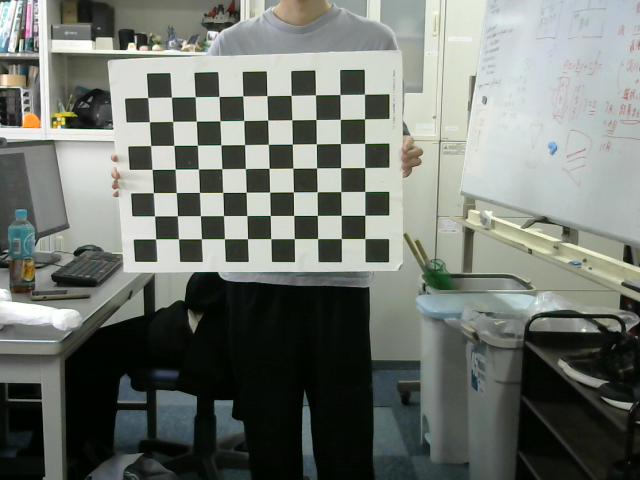
\includegraphics[keepaspectratio, scale=0.1]{figures/carib/camera1/1.png}&
      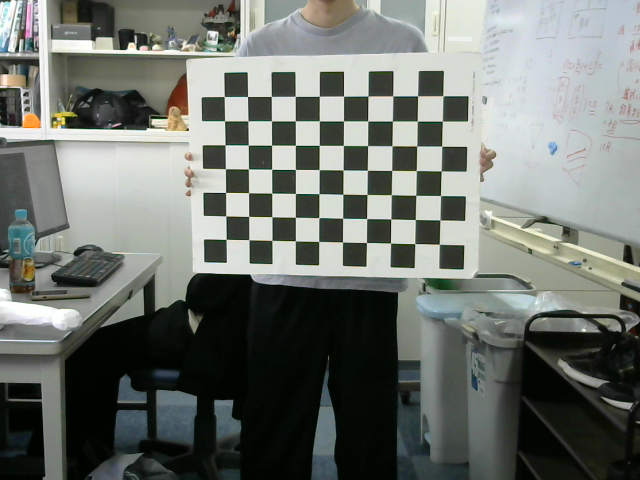
\includegraphics[keepaspectratio, scale=0.1]{figures/carib/camera1/2.png}&
      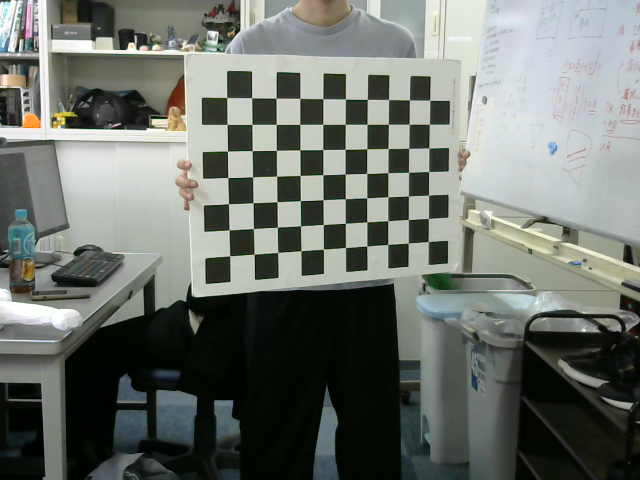
\includegraphics[keepaspectratio, scale=0.1]{figures/carib/camera1/3.png}&
      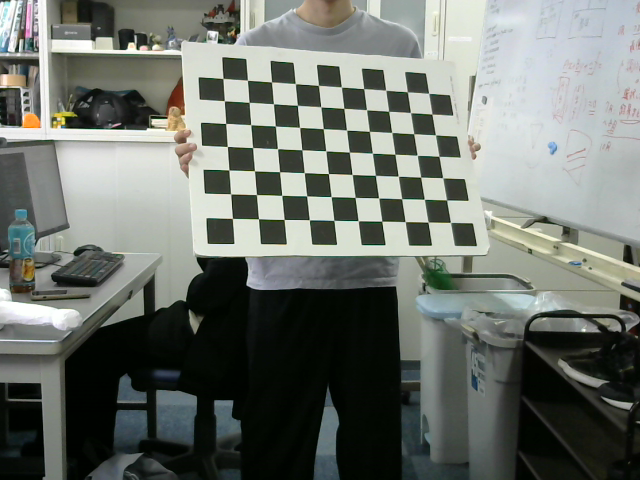
\includegraphics[keepaspectratio, scale=0.1]{figures/carib/camera1/4.png}&
      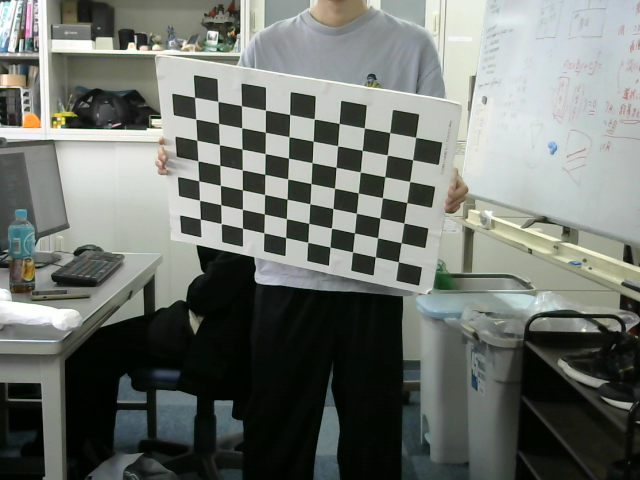
\includegraphics[keepaspectratio, scale=0.1]{figures/carib/camera1/5.png}\\
      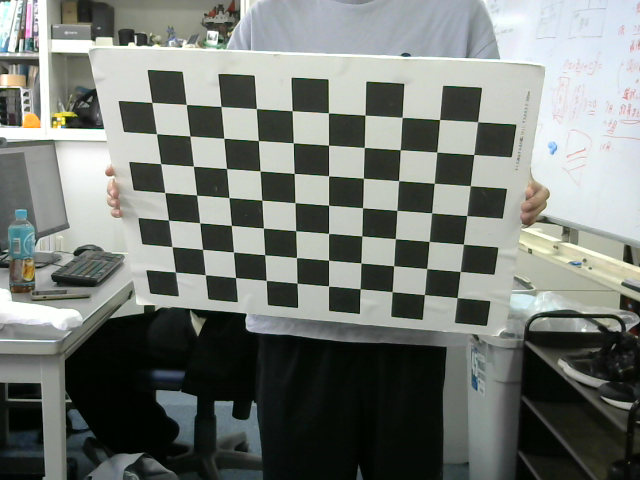
\includegraphics[keepaspectratio, scale=0.1]{figures/carib/camera1/6.png}&
      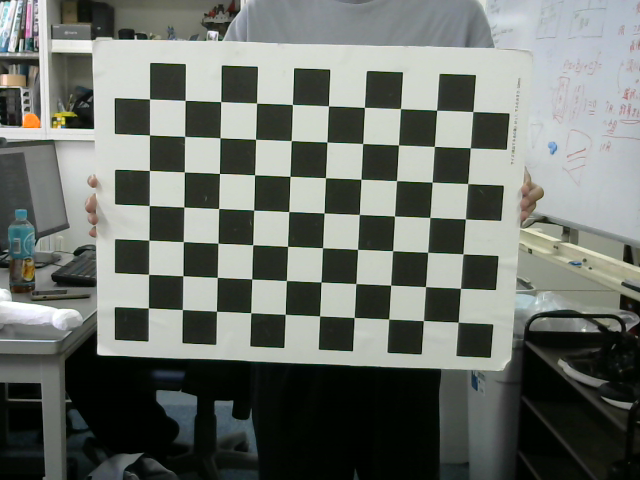
\includegraphics[keepaspectratio, scale=0.1]{figures/carib/camera1/7.png}&
      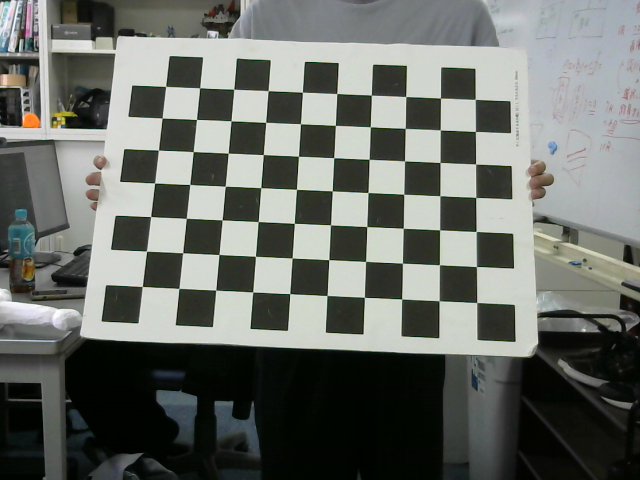
\includegraphics[keepaspectratio, scale=0.1]{figures/carib/camera1/8.png}&
      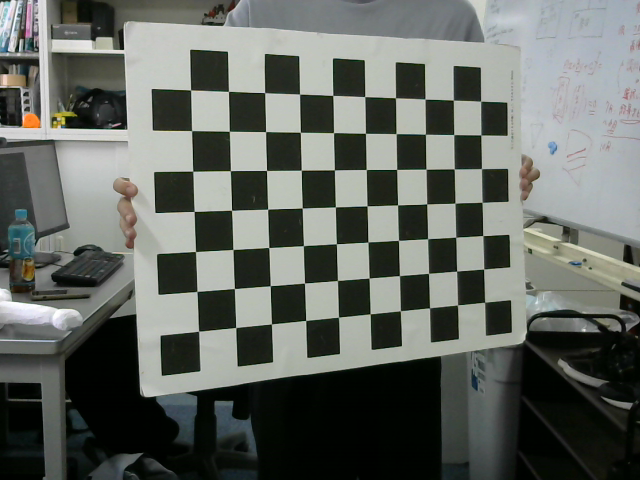
\includegraphics[keepaspectratio, scale=0.1]{figures/carib/camera1/9.png}&
      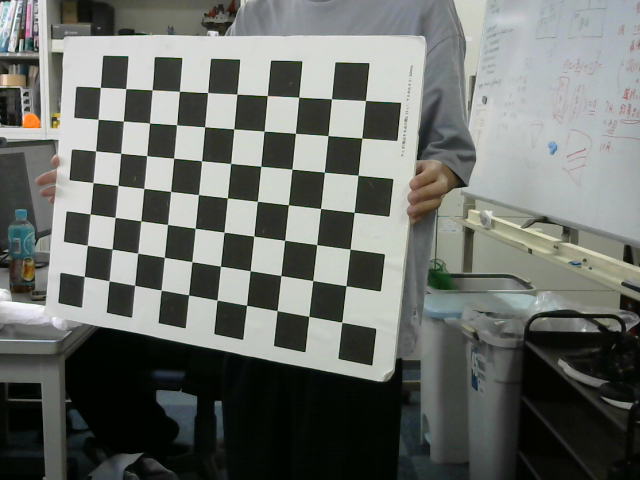
\includegraphics[keepaspectratio, scale=0.1]{figures/carib/camera1/10.png}\\
    \end{tabular}
  \end{center}
  \caption{チェッカーボードの画像1}
  \label{one}
\end{figure}
\begin{figure}[!ht]
  \begin{center}
    \begin{tabular}{ccccc}
      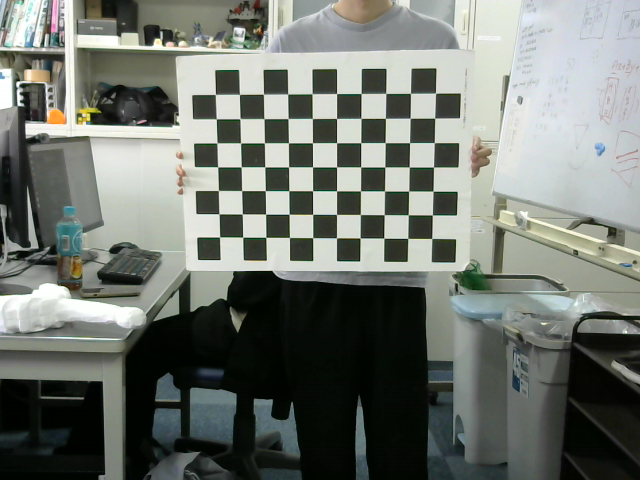
\includegraphics[keepaspectratio, scale=0.1]{figures/carib/camera2/1.png}&
      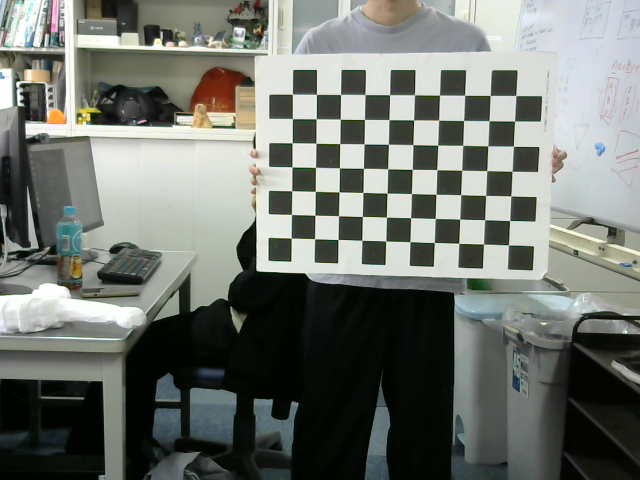
\includegraphics[keepaspectratio, scale=0.1]{figures/carib/camera2/2.png}&
      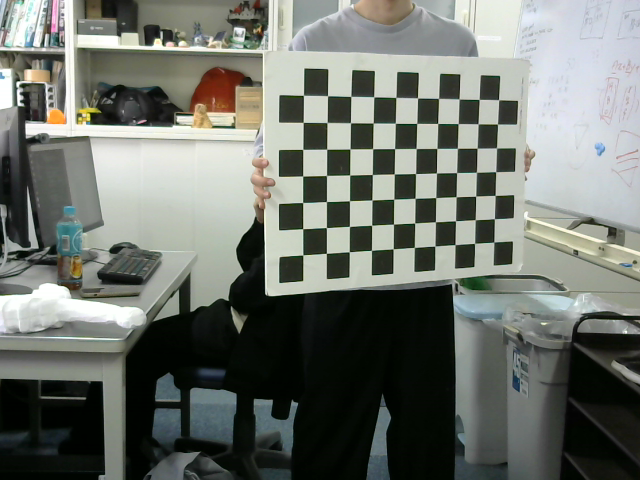
\includegraphics[keepaspectratio, scale=0.1]{figures/carib/camera2/3.png}&
      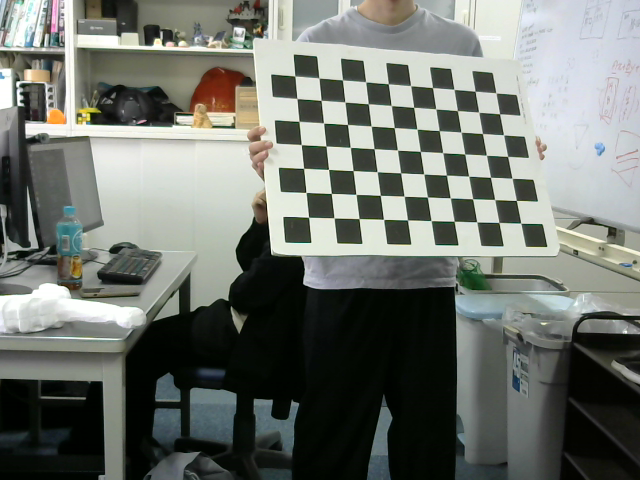
\includegraphics[keepaspectratio, scale=0.1]{figures/carib/camera2/4.png}&
      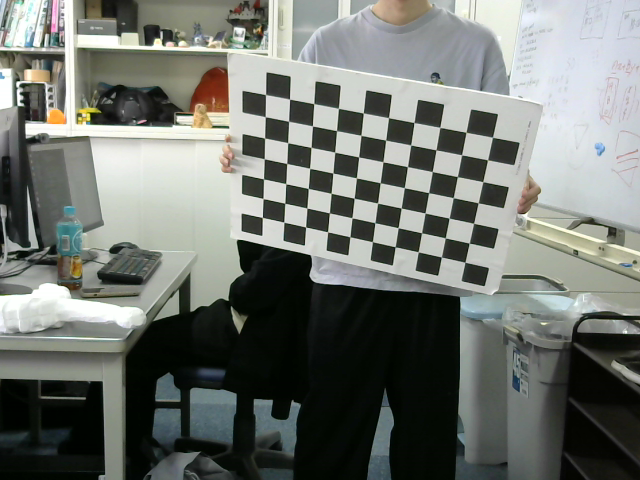
\includegraphics[keepaspectratio, scale=0.1]{figures/carib/camera2/5.png}\\
      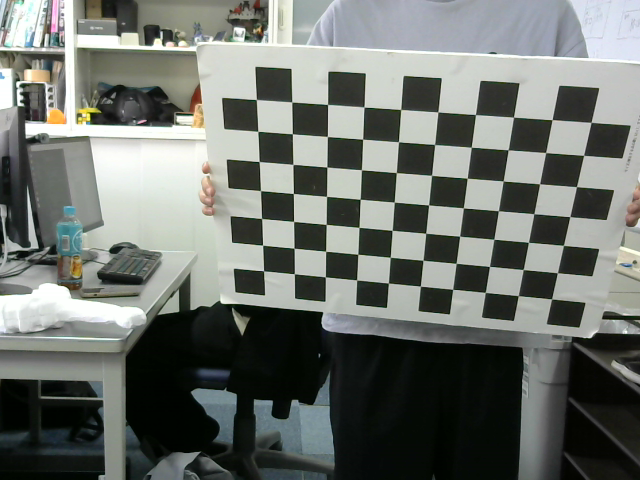
\includegraphics[keepaspectratio, scale=0.1]{figures/carib/camera2/6.png}&
      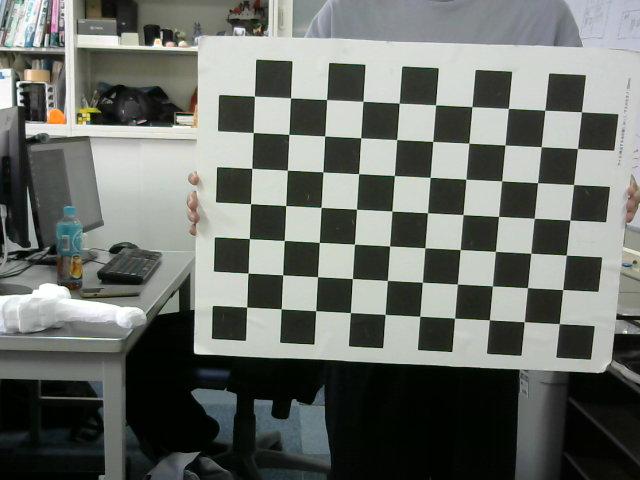
\includegraphics[keepaspectratio, scale=0.1]{figures/carib/camera2/7.png}&
      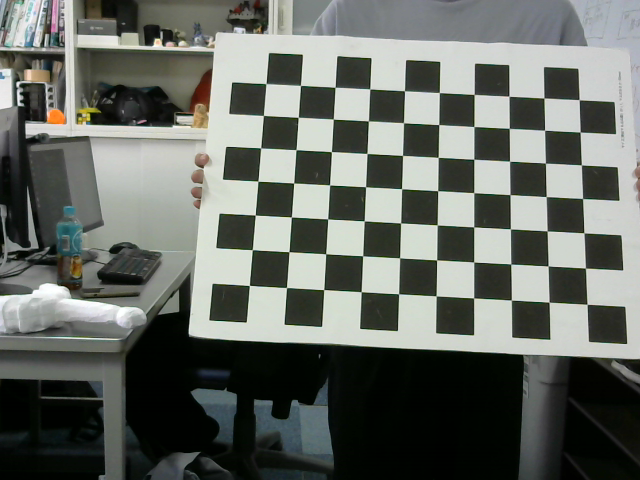
\includegraphics[keepaspectratio, scale=0.1]{figures/carib/camera2/8.png}&
      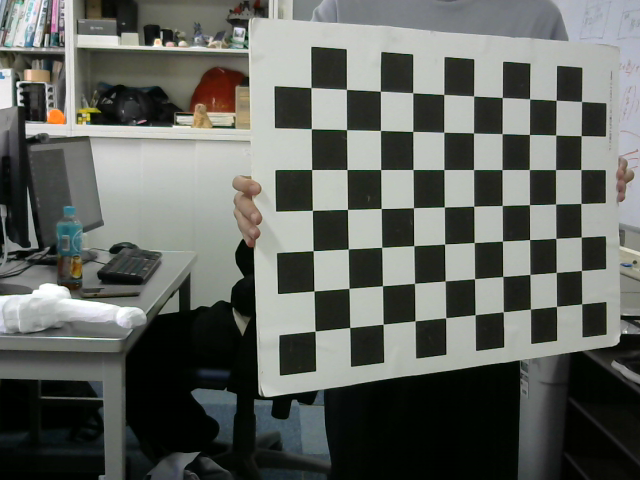
\includegraphics[keepaspectratio, scale=0.1]{figures/carib/camera2/9.png}&
      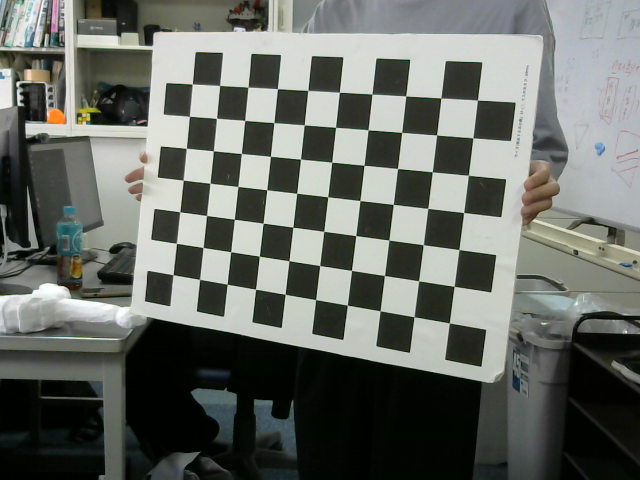
\includegraphics[keepaspectratio, scale=0.1]{figures/carib/camera2/10.png}\\
    \end{tabular}
  \end{center}
  \caption{チェッカーボードの画像2}
  \label{two}
\end{figure}
カメラ1、カメラ2の外部パラメータ、内部パラメータの推定した様子を\hyperref[three]{図\ref{three}}に示す。
\begin{figure}[!ht]
  \begin{center}
    \begin{tabular}{c}
      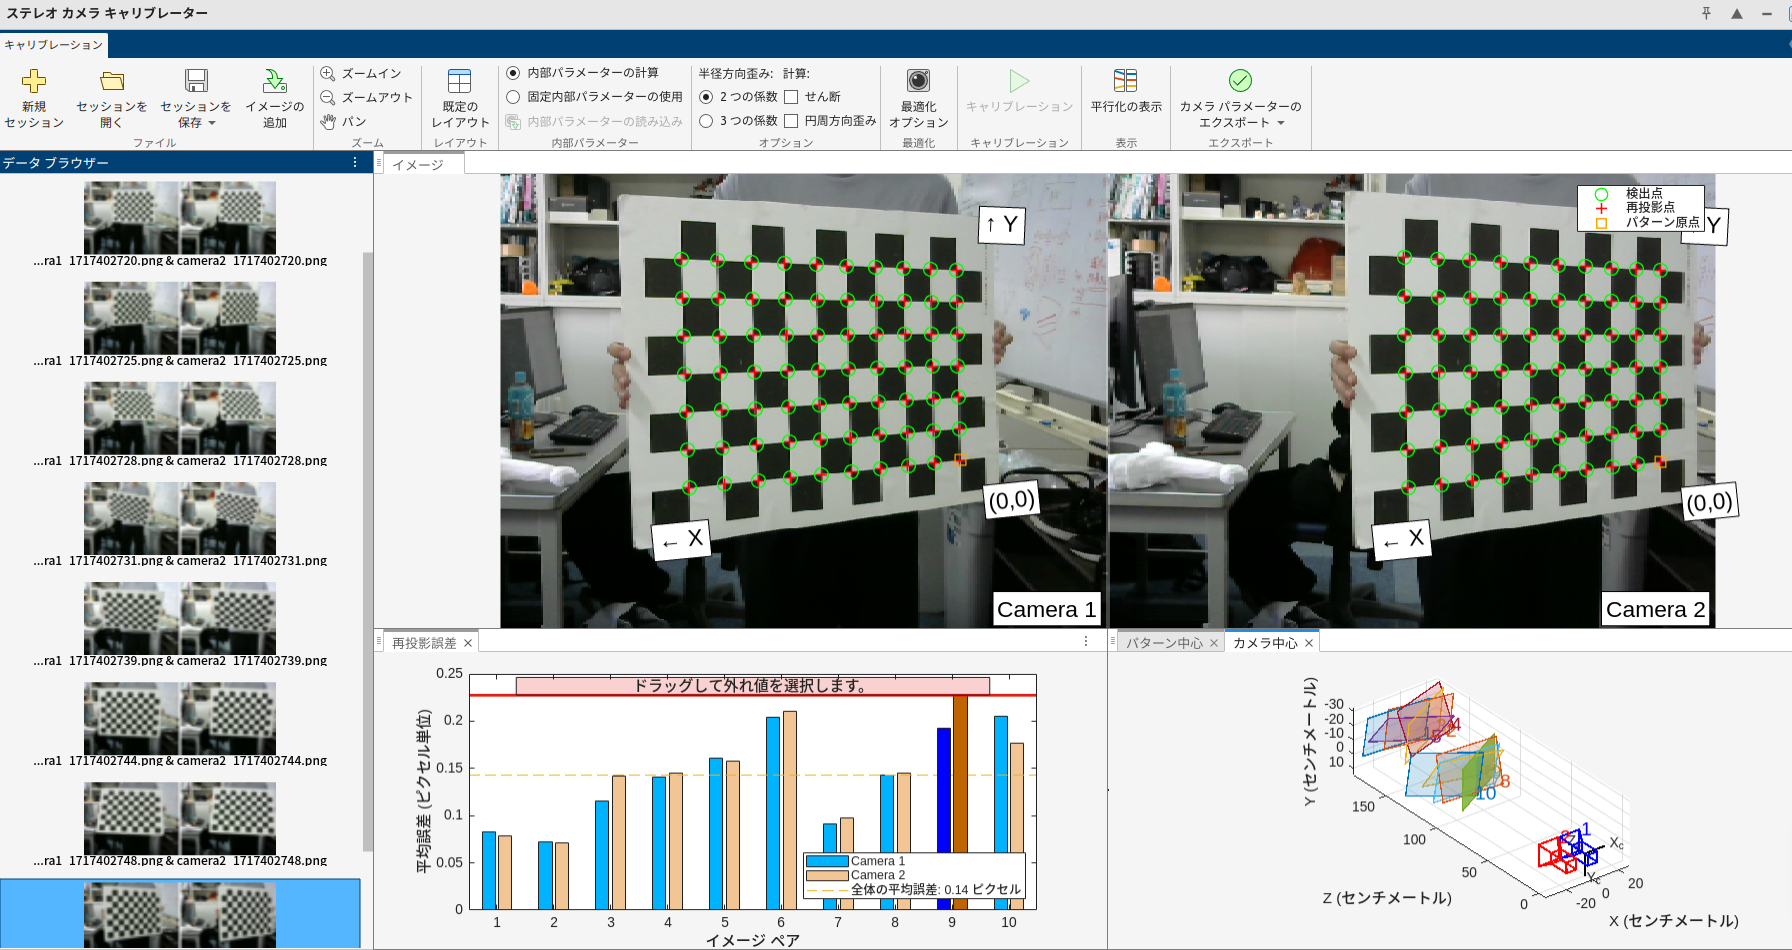
\includegraphics[keepaspectratio, scale=0.2]{figures/stereo.png}\\
    \end{tabular}
  \end{center}
  \caption{カメラのキャリブレーション}
  \label{three}
\end{figure}
カメラとチェッカーボードの位置関係を推測することができているとわかる。
また、カメラの内部パラメータやステレオカメラの基本行列等がstereoParams.matとして出力される。
\subsection{2画像からの3次元復元}
前節で求めたカメラの内部パラメータ、外部パラメータを用いて2画像からの3次元復元を行う。
入力として用いる2つの画像を\hyperref[four]{図\ref{four}}に示す。
\begin{figure}[!ht]
  \begin{center}
    \begin{tabular}{c}
      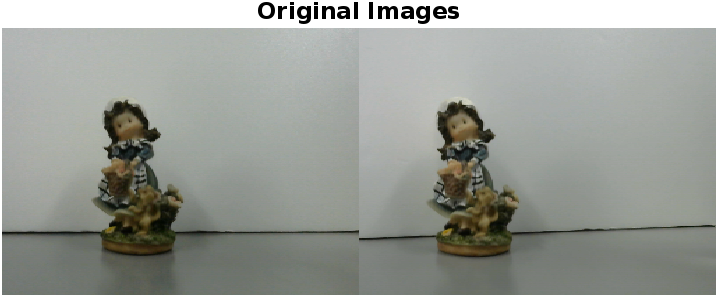
\includegraphics[keepaspectratio, scale=1.0]{figures/1.png}\\
    \end{tabular}
  \end{center}
  \caption{入力画像}
  \label{four}
\end{figure}
\newline
この画像に対して、カメラ1の歪み係数を用いてレンズ歪みを除去する。
実行後の画像を\hyperref[five]{図\ref{five}}に示す。
輪郭付近の一部が削り取られて、歪みが除去されていることがわかる。
\begin{figure}[!ht]
  \begin{center}
    \begin{tabular}{c}
      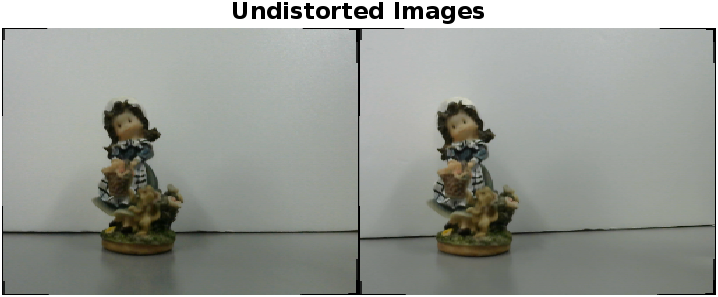
\includegraphics[keepaspectratio, scale=1.0]{figures/2.png}\\
    \end{tabular}
  \end{center}
  \caption{レンズ歪み除去}
  \label{five}
\end{figure}
\newline
次に、画像の特徴点を抽出し、2画像の特徴点を対応付けする。
抽出した特徴点を\hyperref[six]{図\ref{six}}に示す。
復元したい物体だけでなく、背景や輪郭部分に特徴点が取られてしまっていることがわかる。
\begin{figure}[!ht]
  \begin{center}
    \begin{tabular}{c}
      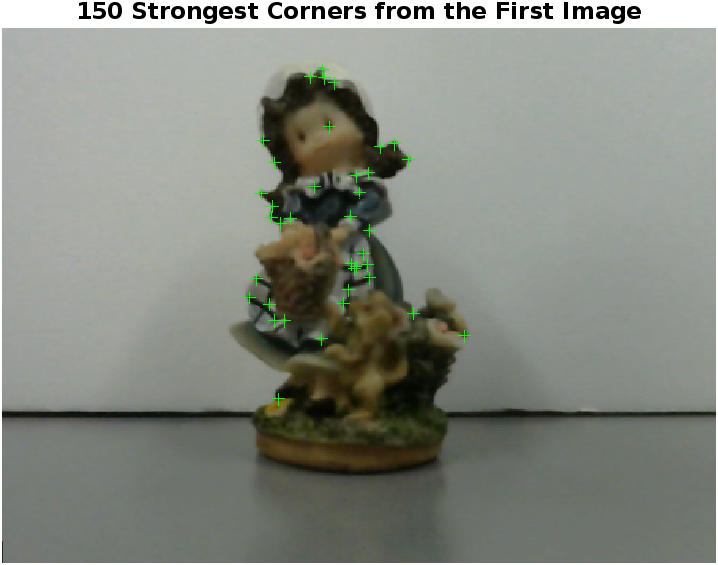
\includegraphics[keepaspectratio, scale=0.9]{figures/3.png}\\
    \end{tabular}
  \end{center}
  \caption{特徴点抽出}
  \label{six}
\end{figure}
\newline
その後、基本行列の推定やカメラ姿勢計算、マッチする点の3次元位置の再構成を行い、
3次元点群として復元する。
復元した画像を\hyperref[seven]{図\ref{seven}}に示す。
\begin{figure}[!ht]
  \begin{center}
    \begin{tabular}{c}
      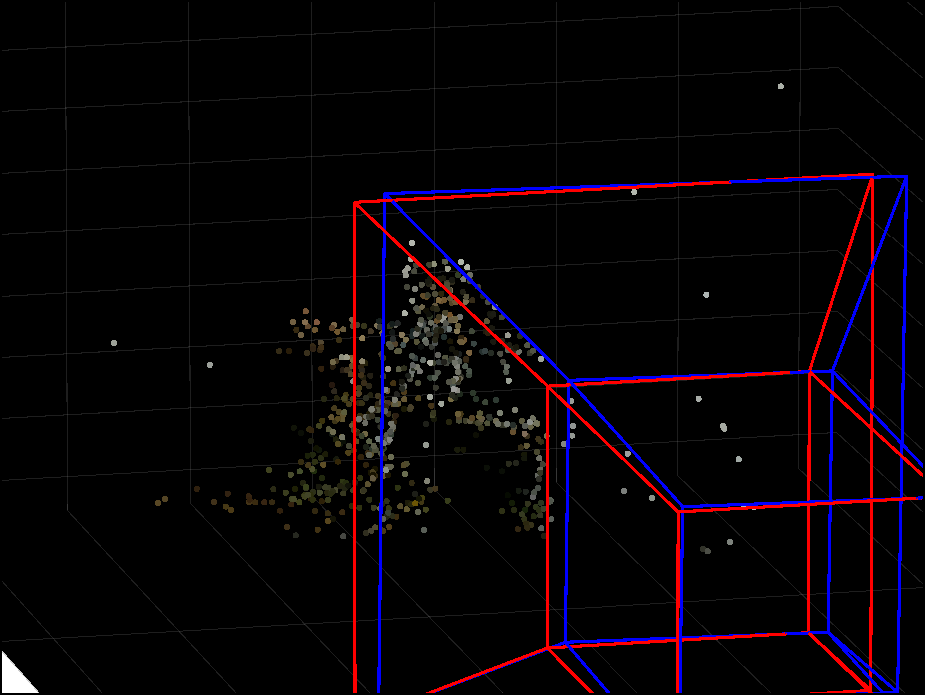
\includegraphics[keepaspectratio, scale=0.7]{figures/7.png}\\
    \end{tabular}
  \end{center}
  \caption{3次元点群による復元}
  \label{seven}
\end{figure}
\newline
ただしmatlabで実行したプログラムについては、付録としてこの資料と共に添付してあるkadai4.mを用いた。
\subsection{考察}
カメラのキャリブレーションについては、matlabを用いてある程度正確にカメラ位置を推定することができた。
2画像からの3次元復元については、完全に復元できたとは言い切れないものになった。
このような結果となった原因について、入力画像の被写体に正しくピントがあっていないことで、
特徴点を多く取れなかったことが考えられる。
また、カメラの画素数が低く、その点も特徴点を多く取れなかったことにつながると考えられる。
改善点として、しっかりピントを合わせて撮影することや、より複数の画像を用いて復元することでいい結果が得られるのではないかと考えた。
\end{document}
